\documentclass[11pt,letterpaper]{article}
\usepackage[margin=0.75in]{geometry}
\usepackage[T1]{fontenc}
\usepackage{lmodern,microtype,amsmath,graphicx}
\usepackage[numbers,sort&compress]{natbib}
\usepackage[colorlinks=true,urlcolor=blue,citecolor=blue,linkcolor=black]{hyperref}
\usepackage{titlesec}
\usepackage{caption}
\usepackage{float}
\titleformat{\section}{\normalsize\bfseries}{}{0pt}{}
\titlespacing*{\section}{0pt}{7pt}{3pt}
\captionsetup{font=small,labelfont=bf,skip=3pt}
\setlength{\parindent}{0pt}
\setlength{\parskip}{3pt}
\setlength{\bibsep}{1pt}
\setlength{\textfloatsep}{8pt}
\setlength{\intextsep}{7pt}
\setlength{\emergencystretch}{2em}
\providecommand{\doi}[1]{\href{https://doi.org/#1}{doi: #1}}
\begin{document}
\begin{center}
{\large\bfseries Predicting Gene-Pair Responses Beyond Additivity\par
with Biological Embeddings and Set Attention\par}
\vspace{3pt}
Pramika Garg \quad | \quad UNI: pg2899 \quad | \quad Interim report
\end{center}
\vspace{-6pt}

\section{Introduction}
Predicting how gene targets act together could help prioritize combinations for therapy. Joint activation can reinforce or suppress responses and alter differentiation~\cite{norman2019}. I ask whether biological gene features and attention improve predictions for unseen combinations. The main comparison is additivity: adding measured single-gene effects. Ahlmann-Eltze et al. found this approach outperformed the deep-learning methods they tested~\cite{ahlmann2025}. I compare it with GEARS~\cite{roohani2024} and an extension using DepMap features and set attention (Fig.~\ref{fig:workflow}). These K562 leukemia-cell experiments can inform target prioritization, but cannot establish drug efficacy.

\begin{figure}[H]
\centering
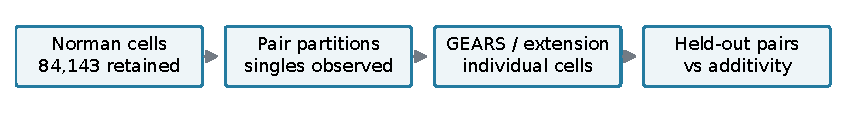
\includegraphics[width=\linewidth]{gpu/figures/01_workflow.pdf}
\caption{Completed workflow. Baselines use five random pair partitions. Both cell-level models share one partition, one initialization and five training epochs.}
\label{fig:workflow}
\end{figure}

\section{Data and exploratory analysis}
I downloaded the scFoundation-processed Norman Perturb-seq release used in~\cite{ahlmann2025}: 84,986 cells, 19,264 genes and 227 conditions. I removed 843 cells from two conditions involving \textit{IER5L}, absent from the supplied Gene Ontology (GO) dictionary. This left \textbf{84,143 cells, 100 single-gene conditions, 124 pairs and one control condition}. The control contains 7,275 cells. Conditions contain 46--7,275 cells, with median 281 (Fig.~\ref{fig:eda}A).

I processed the sparse matrix in chunks to calculate condition means, variances and cell summaries. Values were nonnegative and continuous, with \texttt{log1p} metadata. I retained this scale without normalizing again. No stored values were nonfinite; 85.1\% of entries were zero (Fig.~\ref{fig:eda}B). Principal component analysis (PCA) of condition means for the 1,000 highest-mean control genes explains 35.1\% and 22.6\% of variance in its first two components. Single-gene and pair conditions overlap (Fig.~\ref{fig:eda}C). Hemoglobin genes \textit{HBZ}, \textit{HBG2} and \textit{HBG1} have the largest absolute PC2 loadings. This exploratory PCA was not model input.

\begin{figure}[H]
\centering
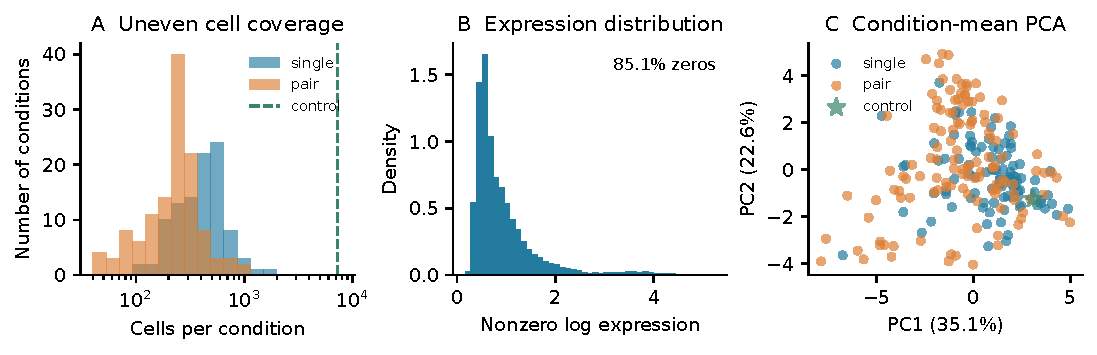
\includegraphics[width=\linewidth]{interim/figures/02_eda.pdf}
\caption{Exploratory analysis. A: cell counts per condition; the dashed line marks the control count. B: sampled nonzero expression values; the zero fraction uses the full retained matrix. C: centered, unscaled PCA of all 225 condition means, colored by condition type.}
\label{fig:eda}
\end{figure}

\newpage
\section{Methods}
\textbf{Withholding gene pairs.} I created five random partitions using seeds 101, 202, 303, 404 and 505. Each assigns 62 pairs to training, 31 to validation and 31 to testing. All single-gene and control conditions remain available for training. Cells from each condition stay together, so a test pair is always unseen as a combination. The five partitions give 155 test appearances covering 98 distinct pairs.

\textbf{Baselines and evaluation.} The additive prediction is $\widehat\mu^{\mathrm{add}}_{AB}=\mu_A+\mu_B-\mu_{\mathrm{ctrl}}$, where $\mu$ denotes mean expression in a condition. Subtracting the control once avoids counting it twice. Two simpler baselines predict the control mean or the equally weighted mean of training perturbation conditions. I measured mean squared error (MSE) on the same 1,000 control-selected genes. Lower MSE means better prediction.

For each pair $p$ in partition $s$, I calculated $D_{p,s}=\mathrm{MSE}_{\mathrm{add},p,s}-\mathrm{MSE}_{\mathrm{model},p,s}$. Positive values favor the model. I averaged repeated test results within pairs, then gave each pair equal weight. Intervals use 10,000 bootstrap resamples of pairs. They describe uncertainty across pairs for these fitted predictors. They do not capture variation from retraining, and overlapping partitions or shared genes do not provide independent biological replication.

\textbf{Neural models.} I trained the pinned upstream GEARS implementation and an extension motivated by MORPH~\cite{he2025}. The extension uses fixed DepMap profiles of gene dependencies across cancer cell lines. It replaces GEARS' sum of gene representations with set attention~\cite{lee2019}. Attention learns how to combine the representations without depending on their order. I used the labeled \href{https://doi.org/10.6084/m9.figshare.21637199}{DepMap 22Q4} release after excluding K562 and its derivative. Features cover 96 of 100 targets. Missing targets receive zero vectors and a presence indicator. A learned projection adds normalized features after the GO encoder; self-attention and learned-seed pooling then combine the target representations. Both models predict all 19,264 genes, use 64 hidden units and the official GO graph of 9,853 nodes. Their coexpression graph uses only individual training cells from single-gene and control conditions.

Both models trained on 67,592 cells. The GEARS loss penalizes the fourth power of expression error and errors in response direction. I used Adam with learning rate $10^{-3}$, weight decay $5\times10^{-4}$, batches of 32 and learning-rate halving each epoch. T4 timing allowed five epochs per model within the shared three-hour budget. Both used partition 101, initialization seed 17 and FP16 precision. Checkpoints were selected using validation data only.

To predict condition means, I used the mean control expression as input and evaluated one condition at a time. At batch size one, this exactly averages predictions over individual control inputs because the input expression enters through a final additive path. I retained upstream graph batching, which can make predictions depend on position within a training batch. This behavior, the processed dataset, short schedule and validation metric limit comparison with published GEARS results.

\section{Preliminary results}
Additivity was the strongest baseline. Across the 98 distinct test pairs, mean MSE was \textbf{0.00929 for additivity}, 0.0206 for the training mean and 0.0364 for the control mean (Fig.~\ref{fig:results}A). Additivity also had lower mean error in each of the five partitions. The training-mean predictor's paired difference was $-0.0113$, with a 95\% interval of $[-0.0139,-0.00872]$.

On the same 31 test pairs in partition 101, MSE was \textbf{0.01098 for additivity}, 0.01375 for GEARS and 0.01985 for the extension (Fig.~\ref{fig:results}B). Both models completed five epochs, and validation selected epoch 3 for each. GEARS beat additivity on 7 of 31 pairs; the extension did so on 6. Their mean paired differences were $-0.00277$ and $-0.00886$. Thus, neither improved on additivity in this run. Because the extension changes both features and aggregation, these results cannot identify either component's separate effect. They also cover only one partition and initialization. Total timed execution was 109 minutes.

I assessed repeatability of responses beyond additivity by independently dividing control, single-gene and pair cells into halves. Across 124 pairs, the median correlation between interaction residuals from the two halves was 0.435. This measures within-screen repeatability, rather than independent biological replication.

\begin{figure}[H]
\centering
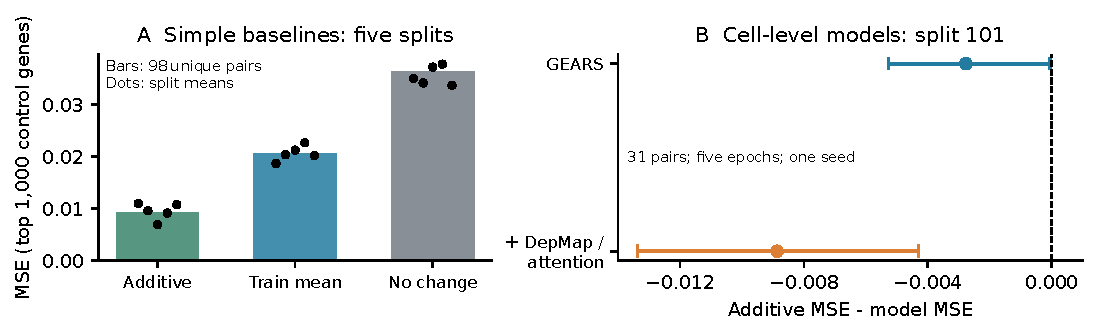
\includegraphics[width=\linewidth]{gpu/figures/03_performance.pdf}
\caption{Prediction performance. A: bars give equal weight to each distinct pair after averaging its test appearances; dots show five partition means. B: additive-minus-model MSE on the same 31 pairs, with 95\% pair-bootstrap intervals. Negative values favor additivity. These intervals do not measure variability across partitions or training initializations.}
\label{fig:results}
\end{figure}

\section{Next steps}
I will repeat training across five partitions and two initializations, assess longer schedules, and separate the effects of gene features and aggregation in the six planned configurations. GenePT~\cite{chen2025} has so far been tested only in earlier models trained on condition means. I will also examine unstable validation errors and the upstream batch-dependent graph implementation. Few combinations, four missing DepMap targets and noisy interaction residuals may make improvements difficult to detect. The prespecified final comparison remains DepMap with attention against additivity, with model selection restricted to validation data. The current results do not establish that embeddings cannot help or that interactions are absent.

\bibliographystyle{abbrvnat}
\bibliography{Interim_Report_References}
\end{document}
